\chapter{Insights}\label{ch:insights}

\section{High Level Usage Stats}\label{sec:high-level-usage-stats}

There is a unavoidable wave of complains that flow in for every assignment in CS-UY 3224
in the day or so before a deadline.
The most common is the classic \textit{you did not give us enough time} excuse,
even if the assignment was assigned weeks before the deadline.

Something unique about spring semester of 2021 for CS-UY 3224 was the introduction of the public usage graph on Anubis.
This graph~\fref{fig:public-usage} is generated every few minutes from live usage data in Anubis.
It shows the number of Cloud IDEs and submissions per hour for each assignment.
Even though it also has the due date for different assignments marked, you could easily deduce the
due date for each.
It is always the day that the usage spikes from basically nothing to hundreds of submissions per hour.

Our response to students asking for extensions was often just showing the usage graphs in lecture.
These graphs are an interesting experiment in student behavior.
They can prove that the majority of students wait until the very last minute to do an assignment
regardless of how long the assignment has been released.
I think most educators have assumed this to be the case, but generating near live graphs from 
this behavior is certainly an unique feature of Anubis.  

\begin{figure}[ht]
    \centering
    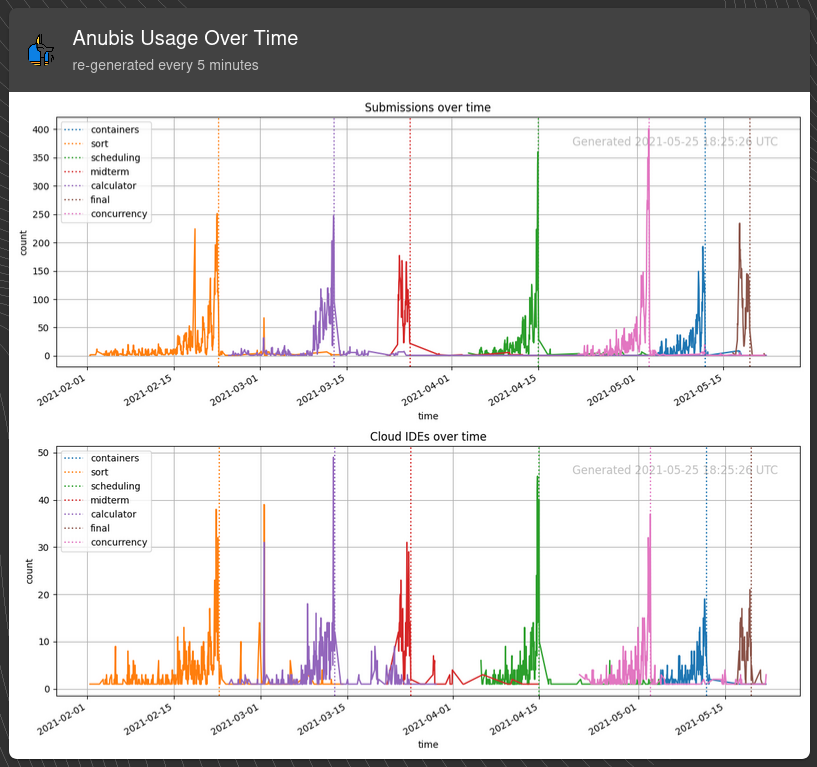
\includegraphics[width=0.5\textwidth]{figures/public-usage-1}
    \caption{Public Usage Graph\label{fig:public-usage}}
\end{figure}

\section{Class Level Autograde Results}\label{sec:class-level-results}

A special visual is generated specifically for visualizing the success of an assignment at a glance.
This visual is called the Anubis Sundial~\fref{fig:autograde-sundial-1}.
It is a radial graph that shows the proportion of students that are passing/failing tests
for a specific assignment.

\begin{figure}[ht]
    \centering
    \begin{subfigure}{0.5\textwidth}
        \centering
        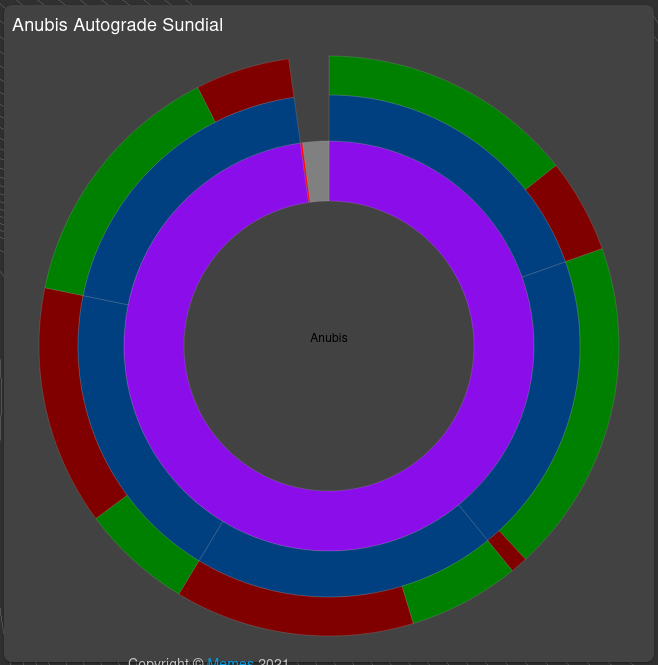
\includegraphics[width=0.9\textwidth]{figures/sundial-1}
        \caption{The Anubis Sundial.\label{fig:autograde-sundial-1} }
    \end{subfigure}%
    \begin{subfigure}{0.5\textwidth}
        \centering
        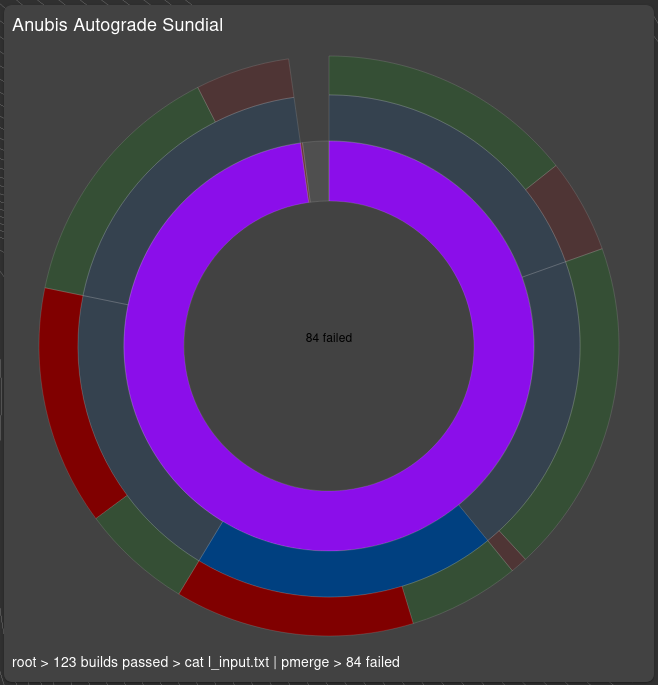
\includegraphics[width=0.9\textwidth]{figures/sundial-3}
        \caption{Many students failed the long file lines test.\label{fig:autograde-sundial-3} }
    \end{subfigure}
\end{figure}

With this simple visualization professors can see which tests students are struggling with.
Sundials are generated live.
At any time, even before the due date, they will be available.
For course administrators, this means that they can see which tests students are struggling with.


Take the simple example in~\fref{fig:autograde-sundial-3}.
By mousing over the sundial, we can see that the tests with long file lines are failing.
This information can then lead to long line buffering being covered again in lecture or
recitation.

\section{Student Level Autograde Results}\label{sec:student-level-results}

Given the structure of Anubis assignments, coupled with the Anubis Cloud IDEs we can
track and measure each student's progress through an assignment with near minute by minute precision.
We can track and measure when students start and finish their assignments,
and how long it takes them to pass specific tests.
In the autograde results panel, a "visual history" is generated for each student.
It shows when students started their assignment, then for each submission if their
build passed or failed and how many tests passed.
If they used the Anubis Cloud IDEs as most students do choose to,
then the graph generated shows a near minute by minute representation of which
challenges they faced and how long it took for them to overcome them.

\begin{figure}[ht]
    \centering
    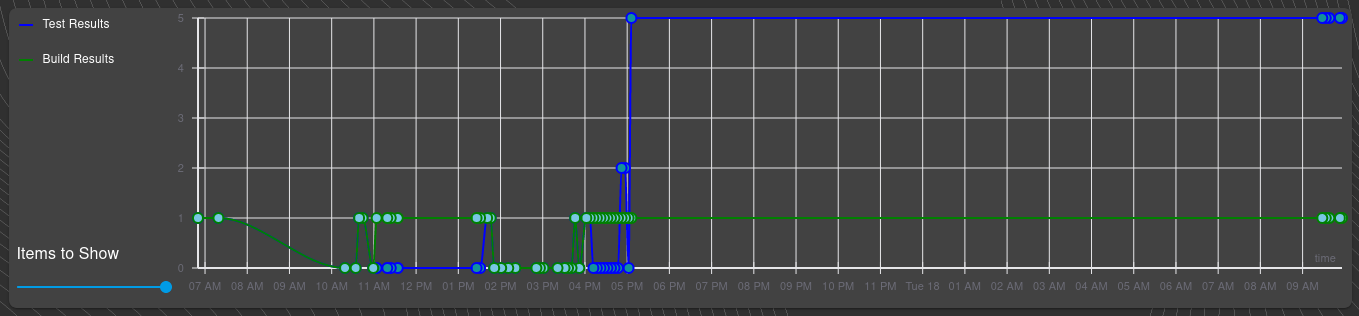
\includegraphics[width=0.9\textwidth]{figures/student-assignment-visual-history-1}
    \caption{A Student Visual History\label{fig:student-assignment-visual-history-1}}
\end{figure}

The example in~\fref{fig:student-assignment-visual-history-1} shows the build as the green
line, and the assignment tests as the blue line.
We can see that this student spent a good deal of time on the first day
just getting their tests to pass, only to revisit their work the next day probably to
clean up their submission.
